
\documentclass[11pt,a4paper]{article}

\usepackage{lmodern}
\usepackage[T1]{fontenc}
\usepackage[utf8]{inputenc}
\usepackage[ngerman]{babel}
\usepackage{microtype}
\usepackage[a4paper,margin=22mm]{geometry}
\usepackage{graphicx}
\usepackage{booktabs}
\usepackage{siunitx}
\usepackage{amsmath}
\usepackage{xcolor}
\usepackage{pgfplots}
\pgfplotsset{compat=1.18}
\setlength{\hfuzz}{1pt} 
\usepackage[hidelinks]{hyperref}

\begin{document}

\section{Auswertung der Test-Session mit EEG Overlay}\label{sec:eeg-session}

\subsection{Aufbau und Zielsetzung}\label{subsec:eeg-aufbau}
Zur explorativen Bewertung des Nutzer Engagements der entwickelten
D3.js Visualisierung wurde eine Art Test-Session als Bildschirmaufzeichnung
festgehalten und diese mit einem EEG (Elektroenzephalografie) Messgerät zusätzlich ergänzt.
Beziehungsweise hat ein Teammitglied den Test durchgeführt.
Die Aufzeichnug wurde mit der EEG Messung ergänzt. Die EEG Messung wurde erst in ein Sounddatei formatiert und
anschließend in eine Welle, welche durch den Taster passend über die Aufzeichnung gelegt wurde. Zudem wurde die Gesichtsaufnahme auch noch ergänt.
Das dadurch enstandende Video, steht als Grundgerüst für die Auswertung um zu sehen, bei welcher Interaktionsmöglichkeit verglichen werden um optisch zu sehen,
was einen User besonders beanspruchen kann und wie gut die benutzten Visualisierungen sind.
Im \textit{EEG-Streifen} kodiert jeder vertikale Balken ein detektiertes Frequenzband-Ereignis.

Dabei steht
\textcolor[HTML]{C0392B}{\textbf{rot}} für \mbox{Alphaaktivität}
(\SIrange{8}{13}{\hertz}, entspannte Wachheit) und
\textcolor[HTML]{2C6FBB}{\textbf{blau}} für \mbox{Betaaktivitärt}
(\SIrange{13}{30}{\hertz}, aktive Konzentration bzw.\ kognitive Verarbeitung).
Ein gelber Streifen markiert die aktuelle Wiedergabeposition, während der
Streifen darunter hinwegläuft. Dadurch lassen sich die Alpha-/Beta-Wellen sehr gut unterscheiden.

Zusätzlich wurde eine Auswertung, welche in der Vorlesung besprochenwurde mit ausgewertet.

\subsection{Methodik}\label{subsec:eeg-methodik}
Der gelbe Streifen steht konstant in der horizontalen Bildmitte
($x_{\text{ph}} \approx \SI{959}{px}$). Der farbcodierte Streifen befindet sich im
vertikalen Bildbereich $y \in [\,860,\,1015\,]\,\si{px}$. Das Video wird im
Zwei Sekunden Raster abgetastet, woraus $N = 170$ St\"utzstellen
$t_k$ resultieren. F\"ur jede St\"utzstelle wird ein schmales Fenster
$\mathcal{W}_k$ um den gelbe Streifen betrachtet
($x \in [\,x_{\text{ph}}-22,\,x_{\text{ph}}+22\,]$, gesamte Streifenh\"ohe).
Innerhalb von $\mathcal{W}_k$ wird jeder Bildpunkt anhand seiner RGB Werte
$(r,g,b)$ als rot  bzw.\ blau dominant klassifiziert:
%
\begin{align}
  \text{rot:}  \quad & (r > 110) \;\wedge\; (r-g > 35) \;\wedge\; (r-b > 30), \\
  \text{blau:} \quad & (b > 110) \;\wedge\; (b-r > 25) \;\wedge\; (b-g > 0).
\end{align}
%
Mit den Pixelz\"ahlern $n^{\alpha}_k$ (rot) und $n^{\beta}_k$ (blau) ergeben sich
je St\"utzstelle der relative Alphaanteil sowie ein dimensionsloses
Aktivit\"atsmaß (Balkendichte, bezogen auf die Fensterfl\"ache
$|\mathcal{W}_k|$):
%
\begin{equation}
  A_k \;=\; \frac{n^{\alpha}_k}{n^{\alpha}_k + n^{\beta}_k},
  \qquad
  D_k \;=\; \frac{n^{\alpha}_k + n^{\beta}_k}{|\mathcal{W}_k|}.
  \label{eq:alpha-activity}
\end{equation}
%
Der Betaanteil folgt komplement\"ar als $B_k = 1 - A_k$. W\"ahrend $A_k$ die
\emph{Balance} der beiden B\"ander beschreibt, erfasst $D_k$ das \emph{absolute
Aufkommen} detektierter Ereignisse und dient als Indikator f\"ur die kognitive
Gesamtlast.

\paragraph{Anmerkung zur Zeitbasis.}
Die $x$-Achse des Streifens l\"auft nicht synchron zur Echtzeit, sondern mit
ann\"ahernd dem Vierfachen. Bei Video Sekunde~\num{200} zeigt der Streifen den
Wert~$\approx\!\num{800}$, bei Sekunde~\num{335} den Wert~$\approx\!\num{1340}$
(Verh\"altnis konstant~$\approx\!4$). Die Streifenachse entspricht somit
vermutlich einer Fenster- bzw.\ Epochenz\"ahlung und nicht physikalischen Sekunden.
S\"amtliche Zeitangaben dieses Abschnitts beziehen sich daher konsistent auf die
\emph{Video Wanduhr} (Session Minuten) und nicht auf die Streifenachse.

\subsection{Ergebnisse}\label{subsec:eeg-ergebnisse}
\"Uber die gesamte Session \"uberwiegt Alpha mit rund \SI{60}{\percent} gegen\"uber
\SI{40}{\percent} Beta. Der Verlauf ist jedoch deutlich strukturiert und l\"asst
sich entlang des sichtbaren Interaktionsmusters in drei Phasen gliedern
(Abbildung~\ref{fig:eeg-timeline}, Tabelle~\ref{tab:eeg-phasen}).

\begin{figure}[htbp]
  \centering
  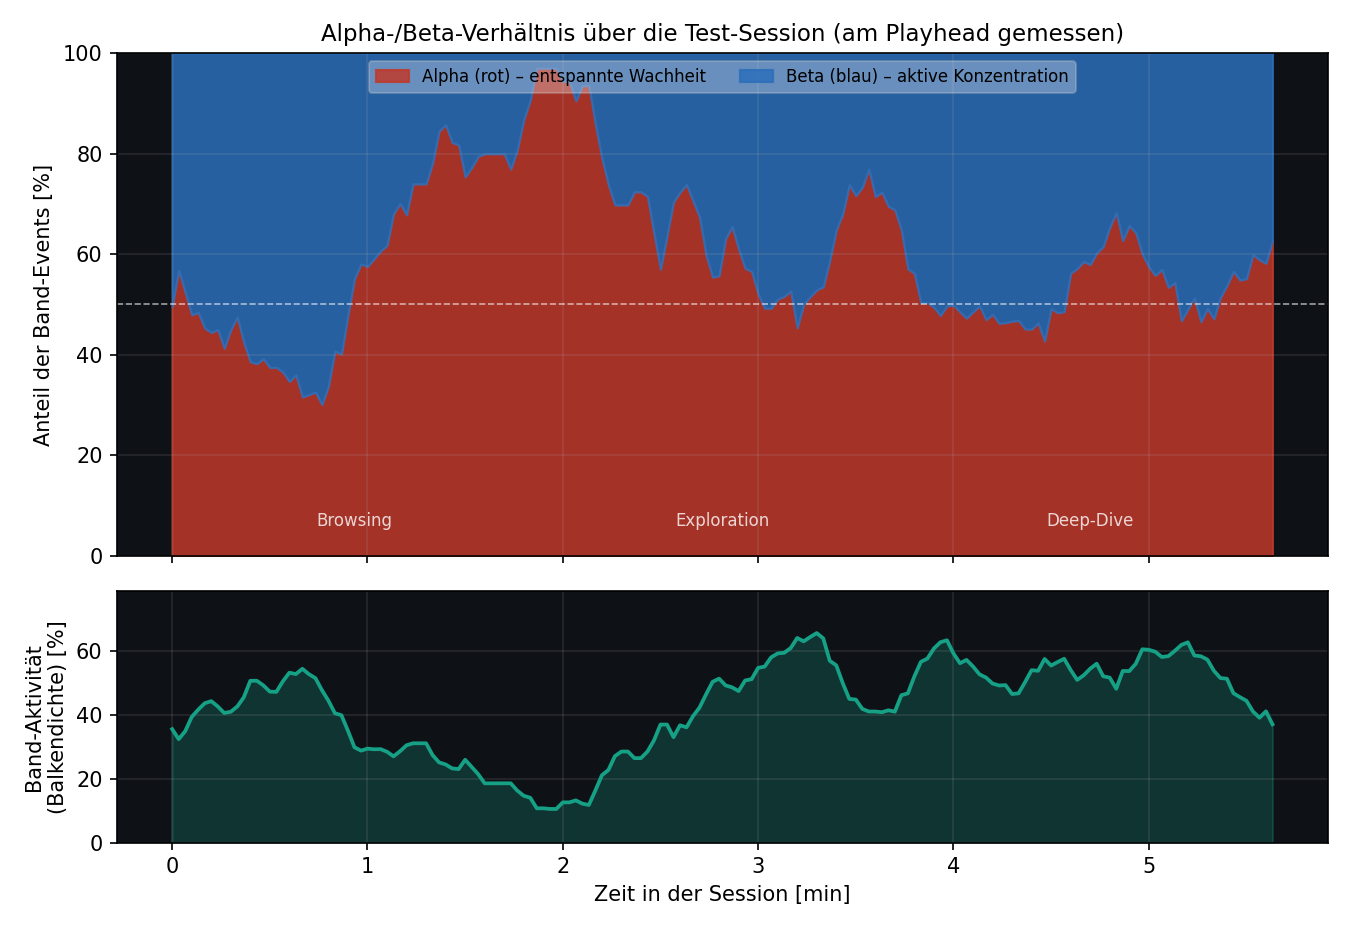
\includegraphics[width=\linewidth]{eeg_profile.png}
  \caption[Alpha/Beta- und Aktivit\"atsverlauf der Test-Session]{%
    Oben: Alpha-/Beta-Verh\"altnis \"uber die Session (rot = Alpha,
    blau = Beta; gestrichelt = \SI{50}{\percent}-Linie). Unten: Gesamtbandaktivit\"at
    $D_k$ (Balkendichte). Die Phasen-Beschriftungen folgen dem sichtbaren
    Interaktionsmuster.}\label{fig:eeg-timeline}
\end{figure}

\begin{table}[htbp]
  \centering
  \sisetup{table-format=2.0}
  \setlength{\tabcolsep}{5pt}\small
  \begin{tabular}{@{}l l S S S@{}}
    \toprule
    \textbf{Phase (Session-Zeit)} & \textbf{Sichtbarer Inhalt}
      & {\textbf{Alpha}\,[\si{\percent}]}
      & {\textbf{Beta}\,[\si{\percent}]}
      & {\textbf{Akt.}\,[\si{\percent}]} \\
    \midrule
    1~-- Browsing \mbox{(0:00--1:53)}     & Dashboard, Heatmap, Shapes      & 58 & 42 & 35 \\
    2~-- Exploration \mbox{(1:53--3:46)}  & ruhiges Betrachten, 3D Skyline  & 69 & 31 & 39 \\
    3~-- Deep-Dive \mbox{(3:46--5:39)}    & UAP-Seiten, Treemap (USA$\to$CA)& 53 & 47 & 54 \\
    \midrule
    \multicolumn{2}{@{}l}{\textbf{Gesamt}} & 60 & 40 & 42 \\
    \bottomrule
  \end{tabular}
  \caption{Phasenweise Mittelwerte des Alpha-/Beta-Anteils und der
  Band-Aktivit\"at~$D_k$.}\label{tab:eeg-phasen}
\end{table}

\begin{figure}[htbp]
  \centering
  \begin{tikzpicture}
    \begin{axis}[
        ybar, bar width=7pt,
        width=0.92\linewidth, height=5.4cm,
        ymin=0, ymax=80,
        ylabel={Anteil / Dichte [\si{\percent}]},
        symbolic x coords={Browsing, Exploration, Deep Dive},
        xtick=data, enlarge x limits=0.28,
        legend style={at={(0.5,1.04)}, anchor=south, legend columns=3,
                      draw=none, /tikz/every even column/.append style={column sep=10pt}},
        ymajorgrids, major grid style={gray!25},
        nodes near coords, nodes near coords style={font=\scriptsize},
        every node near coord/.append style={/pgf/number format/precision=0},
      ]
      \addplot[draw=none, fill={rgb,255:red,192;green,57;blue,43}]
        coordinates {(Browsing,58) (Exploration,69) (Deep Dive,53)};
      \addplot[draw=none, fill={rgb,255:red,44;green,111;blue,187}]
        coordinates {(Browsing,42) (Exploration,31) (Deep Dive,47)};
      \addplot[draw=none, fill={rgb,255:red,22;green,160;blue,133}]
        coordinates {(Browsing,35) (Exploration,39) (Deep Dive,54)};
      \legend{Alpha, Beta, Aktivit\"at}
    \end{axis}
  \end{tikzpicture}
  \caption{Phasenvergleich: Alpha-/Beta-Anteil und Bandaktivit\"at.
  Mit fortschreitender Session sinkt der Alpha-\"Uberhang, w\"ahrend Beta und
  Aktivit\"at im Deep Dive ihr Maximum erreichen.}\label{fig:eeg-bars}
\end{figure}

Eine zentrale Beobachtung betrifft das Zusammenspiel von Balance und Aktivit\"at.
Die \emph{geringste} Gesamtaktivit\"at f\"allt zeitlich mit dem \emph{h\"ochsten}
Alphaanteil zusammen (um Minute~2, Alphaspitze bis~$\approx\!\SI{97}{\percent}$).
In der zweiten Sessionh\"alfte steigt die Bandaktivit\"at hingegen kontinuierlich
von~$\approx\!\SI{15}{\percent}$ auf~$\approx\!\SI{60}{\percent}$, w\"ahrend der
Betaanteil zunimmt. Ein Muster, das auf anhaltende, aktive Verarbeitung
hindeutet.

\subsection{Interpretation entlang der Phasen}\label{subsec:eeg-interpretation}

\paragraph{Phase 1: Browsing / Orientierung.}
Zu Beginn ist Beta leicht erh\"oht (Spitze~$\approx\!\SI{70}{\percent}$ um
Minute~0:50) bei mittlerer Aktivit\"at. Dies deckt sich mit einer
Orientierungsphase. Layout, Heatmap und Shapeverteilung werden erstmalig erfasst,
die hierf\"ur n\"otige visuelle Suche und Einordnung neuer Information beansprucht
aktive Aufmerksamkeit und damit Beta.

\paragraph{Phase 2: Exploration / niedrige Erregung.}
Um Minute~2 dominiert Alpha klar (bis~$\approx\!\SI{97}{\percent}$) bei zugleich
minimaler Gesamtaktivit\"at $D_k$. Der Abschnitt entspricht einem ruhigen, eher
passiven Betrachten. Unter anderem der 3D Skylineansicht, mit geringer
Interaktionsdichte. Hohe Alphaaktivit\"at bei niedrigem Ereignisaufkommen ist als
entspannte Wachheit bzw.\ geringe kognitive Last zu deuten. Der Proband
\"uberfliegt Bekanntes, ohne fokussiert zu arbeiten.

\paragraph{Phase 3: Deep Dive / anhaltende Fokusierung.}
In der zweiten H\"alfte pendelt das Verh\"altnis auf \SI{50}{\percent}, \SI{50}{\percent}.
Der Betaanteil steigt sp\"urbar und entscheidend für die Gesamtaktivit\"at
erreicht ihr Maximum ($\approx\!\SI{60}{\percent}$). Inhaltlich f\"allt dies mit den
informationsdichten, st\"arker interaktiven Teilen zusammen. Dem Durcharbeiten der
UAP Dokumentseiten und dem schrittweisen Hineinzoomen in die Treemap
(Land\,$\to$\,Staat\,$\to$\,Stadt mit mehreren hundert Eintr\"agen).

\paragraph{Zusammenfassende Deutung.}
Die dichten, interaktiven Komponenten der Visualisierung erzeugen messbar
mehr aktive Verarbeitung als das
initiales Überblicksbrowsing oder das ruhige Betrachten der statischen Diagramme.
Aus Perspektive die Fokusierung des Users zu maximieren sind somit gerade die explorativen Elemente
(Treemap Deep Dive, Dokumentrecherche) die Stärke der Auswertung des Datensatzes.

\end{document}